\chapter{Development of the new test network}


\section{Network installation}

For the network, I used GL-AR750 for the main site and GL-AR150 for the remote sites. There are not much work to do on the remote site. We just want to disable the DHCP on the LAN interfaces (because it will get an IP address and not distribute them).

For the two GL-AR750, we have a bit more work to do. We have two different routers to configure:
\begin{itemize}
	\item The master router who will distribute the IP addresses and control the network
	\item The slave router who will extend the master router's network and act as a bridge
\end{itemize}

\subsection{Master router configuration}

For the master router, we need to configure:
\begin{itemize}
	\item The LAN network (Wi-Fi and ethernet)
	\item The fixed addresses
\end{itemize}


We create a Wi-Fi network. It will be easier to use. Indeed, you don't need any cable and can connect your computer to the network wireless. We use fixed IP addresses and names for the remote routers. If they have fixed names, they will be easier to find for our client.


\subsection{Slave router configuration}

For the slave router, we need to configure the bridge function. The problem is that the GL-AR750 can not by default make a bridge between two Wi-Fi interfaces. He can bridge a Wi-Fi interface with an ethernet one or bridge two ehternet interfaces but not two Wi-Fi interfaces. Thankfully, a workaround exists. Indeed, there is package called relayd. This package lets you simulate a bridge behaviour. In fact, this package will transform our router into an invisible bridge. The devices that connect to the slave router, it will be like they are connected to the master router.


\begin{figure}[H]
\begin{center}
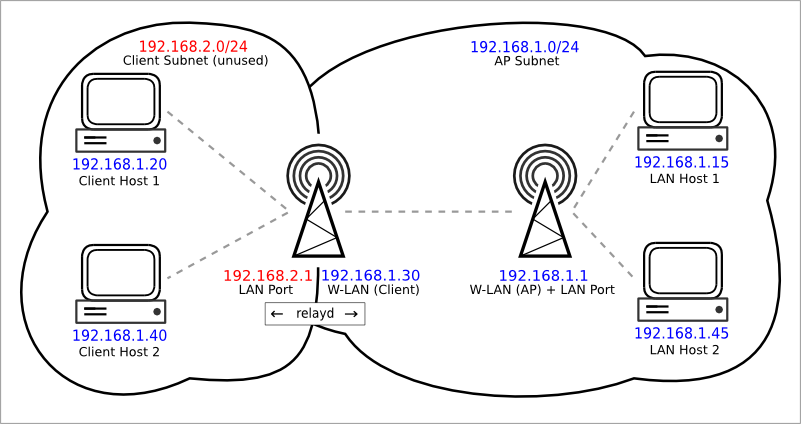
\includegraphics[width=0.7\textwidth]{image/802-11-routed-relay.png}%
\caption{Bridge network with relayd (source: https://wiki.openwrt.org/doc/recipes/relayclient)}%
\label{figure:relayd}%-
\end{center}
\end{figure}

We have two networks, one in blue and one in red. The master router is the one on the right (192.168.1.1). He is controlling the blue network. The slave router is connected to the master router. It is controlling the red network. We need to create this network for relayd but it is not really used. As you can see on the figure, the devices connected to the slave router are using addresses belonging to the blue network. For them, the slave router is just a bridge and does not really exist.





\section{Development of the server}

The server is a TCP server coded in C. It uses the LBARD code made by the Serval team. In particular, we are interested in one driver in the LBARD code. Indeed, the server needs to communicate with the RFD900+. 

\subsection{Building a TCP server}
The first thing I developed was the  TCP infrastructure of the server.
The infrastructure of the server is the following:
\begin{itemize}
	\item We first transform the server into a daemon (a daemon is process running in the background. It is not linked to a terminal and it can't print any data on the screen)
	\item We initialise the TCP socket
	\item We bind the socket
	\item We start listening on the socket to see incoming clients
	\item We have a while loop to accept any client
\end{itemize}

The while loop is where we handle the incoming client. In this loop the server wait for a client.
When receiving a client, the server will create another process (a child).
The main process will stay in the while loop to accept other client.
The child will exit the while loop and start communicating with the client. A communication in TCP is very basic.
You can either send data or receive data but you cannot do both at the same time. One thing to be aware is if the server tries to receive a message using the c function called "recv", he will be stuck until it actually receives a message.
So we need to make a choice. To do that, we can use the function called "poll". This function lets you analyse many sockets to see if one of them has received something. You precise a timer during which the function will look at the sockets. If a message is received on a socket, the poll function will end and tell you which socket has received a message. In this case, the child process will receive the message, understand it, and execute the correct part of the code. For instance, if it receives a "STOP" message, the child process will stop the communication and end.

If no message is received, the timer of the poll function will run out. In this case, the child process will send data to the client.

By default, the data sent are the UHF messages of the Mesh Extender.



\subsection{Integrating the LBARD code}

We want to send UHF messages. But, by default, the GL-AR150 does not have a radio interface able to perceive them. That's why we are using a RFD900+. To use it, we need to understand it using a driver. Paul developed a C driver for the RFD900+. Furthermore, the LBARD code is using this driver and is able to understand the RFD900+. So for my server, I reused the LBARD code made by the Serval team. Using all the needed files, I adapted them for the server.

I earlier explained that the first step of the server is to transform itself into a daemon. A daemon can not print data to the screen because it is not linked to any terminal and it doesn't have any standard output. However, the LBARD code is printing a lot of data. We need to remove all these printing. Instead of printing, we want to send them on the network to the client.
We have two solutions for that:
\begin{itemize}
	\item solution 1: Modify each function of the LBARD code to replace all the printing functions by using the function called "send". 
	\item solution 2: Redirect the standard output to the socket. It will mean that every function trying to print data will instead send them to the client  
\end{itemize}

The first solution is cleaner but very time consuming. The second solution is easier, faster and if someone want to add code to the server, he can do that without having to worry about the TCO aspect.

I actually implemented both solution. I modified a lot of the LBARD functions so they don't print data but rather send them. And as a backup for any mistake I could make and for the future users, I redirected the standard output to the network socket.




\section{Development of the client}

The client part is made of two programs: the client and the client\_shell.

\subsection{Development of the client}
The client is a basic TCP client that can also receive orders from the client\_shell.

First, need to prepare the client to receive orders from the client\_shell.
Since both programs are on the same computer, we can use named FIFO. A FIFO is a pile where you can store data, and they will be read in the same order as they have been put in the FIFO.
The client will open the named FIFO. The named FIFO was created by the client\_shell.
If the client was launched by the client\_shell, he will know the name of the FIFO and opened it. If the client was manually launched by the user, it will have no FIFO and will use the standard input to receive orders.



We now need to develop a basic TCP client:
\begin{itemize}
	\item We start by creating the socket
	\item We connect to the server
\end{itemize}
 
We are now ready to receive and send messages. But, in the same way as the server, the client needs to choose one option. This time, it will have to choose between:
\begin{itemize}
	\item Receiving data from the server
	\item Receiving orders from the client\_shell or the user
\end{itemize} 

We can once again use the function "poll". This function can look at any file descriptor to see if there is something to read. Thankfully, on Linux, everything is a file. So both the socket, the standard input and the named FIFO have file descriptors.
So we do a poll over these files descriptors and see which one has received something.

If the named FIFO (or the standard input) have received something, the client will read the order and execute. Right now, there are two possible orders:
\begin{itemize}
	\item "STOP" to close the connection. In this case, the client will send a "STOP" to the server to inform him
	\item "LOG" to start or stop logging the data received from the server
\end{itemize}

If the client received a message from the server, he will read the data and print them. It will also log them if it has received the order.

If both sockets have a message to read, the client will prioritise the order from the client\_shell.


Finally, I have added one functionality to the client. If the user tries to stop it without using the "STOP" message, the client will detect it (try to detect it) and send a "STOP" message to the server before stopping.


\subsection{Development of the client\_shell}

The client\_shell is a shell-like interface. To developed that interface I used the following tutorial: \url{https://brennan.io/2015/01/16/write-a-shell-in-c/}.

It explains how to create a shell in c and how to add built in functions.

So in this shell, we have two types of function:
\begin{itemize}
	\item Built in functions: function I have created. They are directly linked to the functioning of the test network.
	\item Classic shell functions
\end{itemize}

The available built in functions are:
\begin{itemize}
	\item help: list the available built in functions
	\item exit: close the client\_shell
	\item launch: launch a client
	\item findServers: update the list of available servers
	\item displayServers: display the available servers
	\item close: close a client
	\item list: list the clients currently running 
	\item log: start or stop logging the data for one client
\end{itemize}

All these functions are made so anyone can use the test network. You don't need to know how it work. With these functions, you have an easy access to the test network.

Let's explain some of them.

\hfill \break \underline{\large{\textbf{findServers}}}

The client\_shell is using a file containing all the possible names of the servers. With this file, he will check which server is available (see if the device is running with a ping). He will add each available server to a list. This function is runned when the client\_shell start to create the list.


\hfill \break \underline{\large{\textbf{displayServers}}}

The client\_shell will print all the servers available (list created by the findServers function). A number is associated to each server. This number can be used by the user to choose a server. The user doesn't have to remember each server address.

\hfill \break \underline{\large{\textbf{launch}}}

launch is used to launch a client. The user needs to precise which server he wants the client to connect to. There are two ways the user can precise the server:
\begin{itemize}
	\item the address of the server
	\item the number precised by the displayServers function
\end{itemize}
When launching a client, the client\_shell will add this client to a list, create the named FIFO and start the client.

\hfill \break \underline{\large{\textbf{list}}}

The function list can be used by the user to see all the clients running. Each client will have a number associated. This number can be used by the user to communicate with the client.

\hfill \break \underline{\large{\textbf{close}}}

The close function can be used to close a client. It will send a "STOP" message to a client. There are two ways of using this function:
\begin{itemize}
	\item Use the number of the client (number found using list) to close this client in particular.
	\item Type "close all" to shutdown all the clients.
\end{itemize}

\hfill \break \underline{\large{\textbf{log}}}

The log function can be used to tell a client to start or stop logging data. Once again, we can use this function in two ways:
\begin{itemize}
	\item "log X filename" to tell the client with the number X to start logging data in a file called filename
	\item "log X stop" to tell the client X to stop logging data
\end{itemize}


\section{Development of the phone and Wi-Fi parts}

Our test network should also monitor the Wi-Fi and allow the user to remotely control the phone.
Right now this two features are still in development. There is a temporary solution for the Wi-Fi and a proof of concept for the mobile part.

\subsection{How to monitor the Wi-Fi remotely}

I wanted to integrate some c code for this part but I unfortunately didn't have the time to do it. Right now, we have to use a temporary solution with the package tcpdump and wireshark (a graphic network tool to analyse messages going through the network).

tcpdump is a Linux package that can be installed on the routers. This package allow an user to scan all the messages going through an interface. Therefore, using this command, we can analyse the Wi-Fi communication going around the router.
We can install this package on the remote router.

Then on the computer in the lab, you simply have to use the following command:

\begin{lstlisting}[language=bash]
ssh root@192.168.8.11 tcpdump -i wlan0 -U -s0 -w - 'not port 22' | ... 
... sudo wireshark -k -i -
\end{lstlisting}

With this command, we launch the command tcpdump on the remote router. It will analyse the Wi-Fi interface called wlan0. Then the result of the tcpdump command is sent to our computer and displayed through wireshark. 


\subsection{How to remotely control a phone}

I managed to remotely control a phone using virtual machines. I had the phone plugged into one virtual machine, and I was controlling the phone in the other virtual machine.

All the component used for this solution were supposed to be available on the small routers. I was hoping it would work smoothly. However, when I tried it on the small routers it didn't work. I still have a proof of concept on virtual machines. It should be possible to make it work on the small router even if it needs to be a little tweaked.

The solution is based on:
\begin{itemize}
	\item adb (android debug bridge) and scrcpy on the computer
	\item usbip on the small router
\end{itemize}

scrcpy is a free open software that use adb to give the user a full control of his phone through a computer. When you launch scrcpy, it will reproduce the screen of your phone on the computer and you can use it.
There is only one issue with scrcpy. It is a very heavy software and can therefore not run on the small routers. 
The solution I came up with was to make scrcpy work on the computer. scrcpy will display the screen of your phone as long as adb can reach it. adb has two ways to reach a phone: through a usb connection or through the network. So I wanted to use the usb connection since the phone will be connected by Wi-Fi to the Mesh Extender and by usb to the remote router. On Linux, there is a package called usbip. This package can make a usb connection work over the network. So we have the phone connected to the remote router using usb. The router transfers this connection to the computer using the network. The computer can use scrcpy to control the phone.



 

